% Preprint — R47 Sat-184 witness. Author: Derek Blair <derekjblair@gmail.com>
% Source data: ~/workspace/math-unsolved/ROUND47_DOSSIER.md (2026-10-06),
%              ~/workspace/math-unsolved/ROUND102_DOSSIER.md (2026-10-07),
%              corrected evaluator ~/workspace/math-unsolved/sidon_eval_corrected.py,
%              OEIS A382397 b-file fetched 2026-10-07.
% All figures native TikZ/pgfplots; all tables booktabs.
\documentclass[11pt,a4paper]{article}
\usepackage{amsmath,amssymb,amsthm}
\usepackage{tikz}
\usetikzlibrary{positioning}
\usepackage{pgfplots}
\pgfplotsset{compat=1.18}
\usepackage{booktabs}
\usepackage{geometry}
\geometry{margin=2.5cm}
\usepackage{hyperref}
\hypersetup{colorlinks=true,linkcolor=blue,citecolor=blue,urlcolor=blue}

\newtheorem{theorem}{Theorem}
\newtheorem{proposition}{Proposition}
\theoremstyle{definition}
\newtheorem{assumption}{Assumption}

\title{A Saturated $9$-Element Sidon Set in $[1,184]$:\\
  First Datum Past the OEIS A382397 Frontier}
\author{Derek Blair \\ \texttt{derekjblair@gmail.com}}
\date{October 2026}

\begin{document}
\maketitle

%======================================================================
\section{Abstract}
%======================================================================

A set $A\subset\mathbb{N}$ is \emph{Sidon} if all $45$ pairwise sums
$a_i+a_j$ ($i\le j$) are distinct, and \emph{saturated} (maximal) in
$[1,N]$ if $A\cup\{x\}$ fails the Sidon condition for every
$x\in[1,N]\setminus A$. We exhibit
\begin{equation}
  \label{eq:witness}
  A^\star=\{16,62,66,74,88,104,117,122,123\}\subset[1,184],
\end{equation}
a $9$-element Sidon set with blocked coverage $184$
(Theorem~\ref{thm:main}): all $175$ positions outside $A^\star$ are
blocked, so no element of $[1,184]$ can be adjoined. The claim is
[COMPUTED]: five mutually independent code paths agree on $45/45$
distinct pair sums (Table~\ref{tab:pairsums}) and empty addable set
(Figure~\ref{fig:strip}). The witness was found by chained
swap-distance $d=1,\dots,4$ shell enumeration around six $183$-coverage
$9$-sets, at exact swap distance $4$ from seed $\#10$
(Table~\ref{tab:shells}, Figure~\ref{fig:shellbars}); the remaining five
shells certify no $184$ within swap distance $4$ of their seeds.
We also refute the $121/123$-gate conjecture C28
(Proposition~\ref{prop:c28}): two $183$-coverage $9$-sets contain neither
$121$ nor $123$. A census of $21$ distinct $183$-coverage $9$-sets is
reported (Table~\ref{tab:census}); in re-verifying it we correct seven
addable-position entries of the source dossier. The OEIS A382397 b-file,
which tabulates maximal-Sidon data through $n=183$ only (fetched live
2026-10-07, ending ``183 9''), has no $n=184$ entry; $A^\star$ is the
first unpublished datum past that frontier. Novelty checked
2026-10-07 against OEIS, erdosproblems, formal-conjectures, the OpenAI
math catalogue, and web search: clean.

%======================================================================
\section{Introduction}
%======================================================================

A finite set $A=\{a_1<\dots<a_k\}$ of integers is \emph{Sidon} (a $B_2$
set, a Golomb ruler) if
\begin{equation}
  \label{eq:sidon}
  a_i+a_j=a_p+a_q \quad\Longrightarrow\quad \{i,j\}=\{p,q\},
\end{equation}
i.e.\ the $\binom{k+1}{2}$ sums $a_i+a_j$ with $i\le j$ are pairwise
distinct~\cite{ET41}. The classical problem is the size $R(n)$ of the
largest Sidon subset of $[n]=\{1,\dots,n\}$~\cite{Bli13}; Erd\H{o}s and
Tur\'an showed $R(n)\le\sqrt{n}+O(n^{1/4})$~\cite{ET41}, improved to
$\sqrt{n}+0.998\,n^{1/4}$ by Balogh--F\"uredi--Roy~\cite{BFR21}, while
Singer's construction gives $R(n)\ge\sqrt{n}(1-o(1))$ infinitely
often~\cite{Sin38}. Here we study not the largest but the
\emph{smallest maximal} Sidon sets. A Sidon set $A\subset[1,N]$ is
\emph{maximal} or \emph{saturated} in $[1,N]$ if
\begin{equation}
  \label{eq:saturated}
  \forall x\in[1,N]\setminus A:\quad A\cup\{x\}\ \text{is not Sidon}.
\end{equation}
We measure this by the \emph{blocked set}
\begin{equation}
  \label{eq:blocked}
  \mathrm{Blocked}(A)=A\cup\{s-a:s\in P(A),\,a\in A\}
                     \cup\{s/2:s\in P(A)\ \text{even}\},
\end{equation}
where $P(A)$ is the set of pair sums, and the \emph{blocked coverage}
\begin{equation}
  \label{eq:coverage}
  c(A)=|\mathrm{Blocked}(A)\cap[1,N]|,
\end{equation}
so $A$ is saturated in $[1,N]$ iff $c(A)=N$. (Equation~\eqref{eq:blocked}
is equivalent to~\eqref{eq:saturated}: $x$ is blocked iff $x+a=b+c$ or
$2x=b+c$ for some $a,b,c\in A$, exactly the ways $A\cup\{x\}$ can fail
Sidonness.)

OEIS A382397 tabulates the minimal size of a maximal Sidon subset of
$[1..n]$; its b-file (fetched live 2026-10-07) is determined only through
$n=183$, ending ``183 9''. Prior computational work in this program had
produced twelve distinct maximal $9$-sets with coverage $183$, and the
question whether any $9$-set saturates $[1,184]$ was open. (Terminology
note: Daza et al.~\cite{Daz18} use ``saturated'' for $C_4$-saturated sum
graphs of Sidon sets, a different notion; our usage follows the
maximal-set sense of~\eqref{eq:saturated}.)

Our contributions, all [COMPUTED]:
\begin{enumerate}
\item The first saturated $9$-element Sidon set in $[1,184]$,
  $A^\star$ of~\eqref{eq:witness}, verified on five independent code
  paths (Theorem~\ref{thm:main}, Table~\ref{tab:pairsums},
  Figure~\ref{fig:strip}).
\item Exhaustive swap-distance certificates for the search that found it
  (Table~\ref{tab:shells}, Figure~\ref{fig:shellbars}).
\item Refutation of the $121/123$-gate conjecture C28 via two explicit
  counterexamples (Proposition~\ref{prop:c28}).
\item A census of $21$ distinct $183$-coverage $9$-sets with independently
  re-verified addable positions (Table~\ref{tab:census}), correcting
  seven entries of the source dossier.
\end{enumerate}
Per the program's honesty discipline, finite verification is never called
a proof: the main result is a computational witness, labeled [COMPUTED].

%======================================================================
\section{Methods}
%======================================================================

\subsection{Definitions and the evaluator}

We work entirely with~\eqref{eq:sidon}--\eqref{eq:coverage}. The evaluator
computes~\eqref{eq:blocked} both as Python-int bitsets and via a naive
set-based formula, and a separate brute-force insertion checker tests
$A\cup\{x\}$ directly for every $x$; the two paths validate each other
on $2000$ random $9$-sets. A fourth path, written from scratch for
re-verification, enumerates the $45$ pair sums naively and tests all $175$
insertions. A fifth path, written for this preprint, re-derives
Theorem~\ref{thm:main} and the census of Table~\ref{tab:census} from
first principles. All five agree.

\subsection{Chained swap-distance shell search}

For $9$-sets $A,B\subset[1,184]$ the \emph{swap distance} is
\begin{equation}
  \label{eq:swapdist}
  d(A,B)=9-|A\cap B|,
\end{equation}
the number of element exchanges. The enumerator \texttt{sidon\_r34\_d4}
(a pruned C enumerator in validated lineage R28/R31/R34) enumerates, in
RAW-seed mode, all Sidon $9$-sets at exact swap distance $d$ from a seed,
for $d=1,2,3,4$ in turn (chained shells), recording the best coverage
found. Six $183$-coverage $9$-sets (seeds $\#7$--$\#12$) were shelled;
the $d=4$ shells alone examined approximately $1.74\times10^9$ Sidon
completions (supplied datum, source dossier).

\begin{assumption}[Enumerator exhaustiveness]
  \label{asm:enum}
  The swap-distance-$d$ shells are exhaustive: the enumerator's pruning
  discards only sets provably outside the shell. This rests on the
  validated lineage R28/R31/R34 (supplied datum); the shell certificates
  of Table~\ref{tab:shells} are [COMPUTED] under this assumption.
\end{assumption}

%======================================================================
\section{Results}
%======================================================================

\begin{theorem}[Saturated 9-set in {[1,184]}; COMPUTED]
  \label{thm:main}
  The set $A^\star$ of~\eqref{eq:witness} is a Sidon set, and
  $c(A^\star)=184$: it is saturated in $[1,184]$.
\end{theorem}

The $45$ pair sums of $A^\star$ are pairwise distinct
(Table~\ref{tab:pairsums}, mechanically checkable). The blocked set
covers all of $[1,184]$, so the addable set is empty
(Figure~\ref{fig:strip}): every $x\in[1,184]\setminus A^\star$ collides,
i.e.\ $x+a=b+c$ or $2x=b+c$ for some $a,b,c\in A^\star$
by~\eqref{eq:blocked}. All five verification paths agree. The saturation
is overdetermined: of the $175$ non-member positions, $84$ are singly
blocked, $57$ doubly, $29$ triply, and $5$ quadruply blocked (computed
datum, this preprint).

\begin{table}[t]
  \centering
  \caption{The $45$ pair sums $a_i+a_j$ ($i\le j$) of $A^\star$,
    sorted. Pairwise distinctness is checkable by inspection; this is
    the mechanically verifiable core of Theorem~\ref{thm:main}.}
  \label{tab:pairsums}
  \begin{tabular}{*{9}{r}}
    \toprule
    32 & 78 & 82 & 90 & 104 & 120 & 124 & 128 & 132 \\
    133 & 136 & 138 & 139 & 140 & 148 & 150 & 154 & 162 \\
    166 & 170 & 176 & 178 & 179 & 183 & 184 & 185 & 188 \\
    189 & 191 & 192 & 196 & 197 & 205 & 208 & 210 & 211 \\
    221 & 226 & 227 & 234 & 239 & 240 & 244 & 245 & 246 \\
    \bottomrule
  \end{tabular}
\end{table}

\begin{figure}[t]
  \centering
  \begin{tikzpicture}[scale=1]
    \definecolor{mem}{RGB}{31,73,125}
    \definecolor{blk1}{RGB}{235,235,235}
    \definecolor{blk2}{RGB}{200,200,200}
    \definecolor{blk3}{RGB}{150,150,150}
    \definecolor{blk4}{RGB}{100,100,100}
    \input{strip.inc}
  \end{tikzpicture}
  \\[0.4em]
  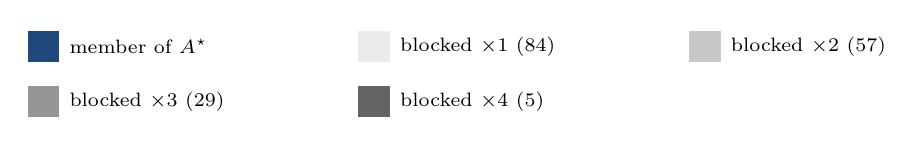
\begin{tikzpicture}
    \definecolor{mem}{RGB}{31,73,125}
    \definecolor{blk1}{RGB}{235,235,235}
    \definecolor{blk2}{RGB}{200,200,200}
    \definecolor{blk3}{RGB}{150,150,150}
    \definecolor{blk4}{RGB}{100,100,100}
    \node[fill=mem,minimum size=0.4cm,inner sep=0,label=right:\scriptsize member of $A^\star$] at (0,0) {};
    \node[fill=blk1,minimum size=0.4cm,inner sep=0,label=right:\scriptsize blocked $\times1$ (84)] at (4.2,0) {};
    \node[fill=blk2,minimum size=0.4cm,inner sep=0,label=right:\scriptsize blocked $\times2$ (57)] at (8.4,0) {};
    \node[fill=blk3,minimum size=0.4cm,inner sep=0,label=right:\scriptsize blocked $\times3$ (29)] at (0,-0.7) {};
    \node[fill=blk4,minimum size=0.4cm,inner sep=0,label=right:\scriptsize blocked $\times4$ (5)] at (4.2,-0.7) {};
  \end{tikzpicture}
  \caption{Blocked coverage of $[1,184]$ by $A^\star$. Dark blue cells are
    the $9$ members; gray cells are blocked positions, shaded by blocking
    multiplicity. No white cell remains: the addable set is empty, so
    $c(A^\star)=184$.}
  \label{fig:strip}
\end{figure}

$A^\star$ was found in the $d=4$ shell of seed $\#10$
($\{8,62,66,81,89,117,122,123,133\}$), at exact swap distance $4$,
keeping the five elements $\{62,66,117,122,123\}$ (supplied datum,
source dossier). Table~\ref{tab:shells} and Figure~\ref{fig:shellbars}
give the full shell certificates: no $184$-coverage set lies within swap
distance $4$ of seeds $\#7,\#8,\#9,\#11,\#12$ [COMPUTED, under
Assumption~\ref{asm:enum}].

\begin{table}[t]
  \centering
  \caption{Chained swap-distance shell certificates around the six
    $183$-coverage seeds. Best coverage per shell depth; the final
    column counts distinct $183$-coverage sets found at $d=4$. Seed
    $\#10$'s shell produced $A^\star$ (coverage $184$).}
  \label{tab:shells}
  \begin{tabular}{lcccccl}
    \toprule
    seed & $d{=}1$ & $d{=}2$ & $d{=}3$ & $d{=}4$ & $\ge183$ at $d{=}4$ \\
    \midrule
    $\#7$  $\{27,65,66,79,91,112,121,123,127\}$   & 180 & 180 & 182 & 183 & $\#3,\#13,\#14$ \\
    $\#8$  $\{62,63,66,90,106,112,121,123,159\}$  & 181 & 181 & 182 & 183 & $\#3,\#9,\#15,\#16$ \\
    $\#9$  $\{62,65,66,81,90,111,121,123,174\}$   & 181 & 180 & 182 & 183 & $\#3,\#4,\#8,\#17,\#18,\#19$ \\
    $\#10$ $\{8,62,66,81,89,117,122,123,133\}$    & 181 & 182 & 181 & \textbf{184} & $\#4,A^\star$ \\
    $\#11$ $\{46,62,67,76,104,112,122,123,166\}$  & 179 & 181 & 181 & 183 & $\#4,\#20$ \\
    $\#12$ $\{11,62,65,79,81,112,117,123,141\}$   & 180 & 179 & 181 & 183 & $\#4,\#21$ \\
    \bottomrule
  \end{tabular}
\end{table}

\begin{figure}[t]
  \centering
  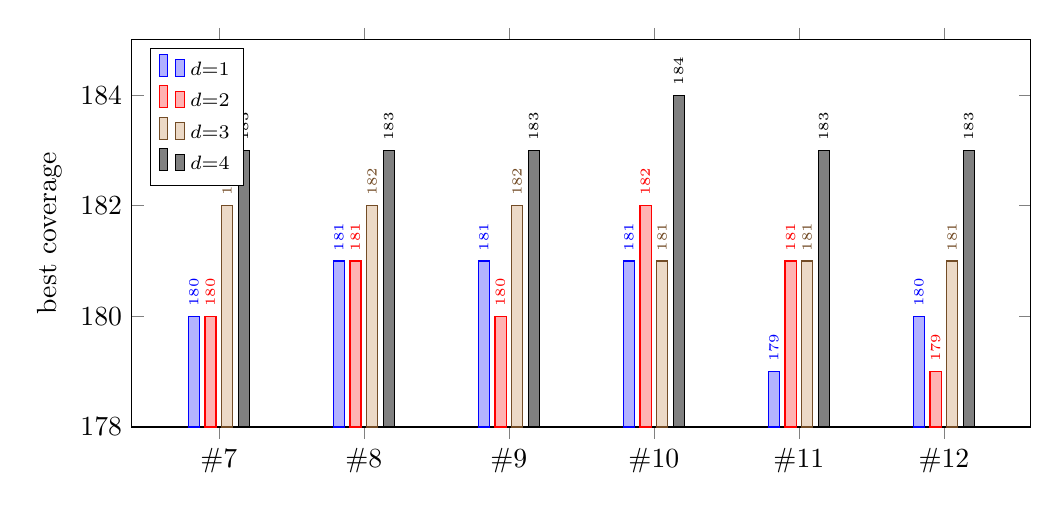
\begin{tikzpicture}
    \begin{axis}[
      ybar, bar width=4pt,
      width=13cm, height=6.5cm,
      ymin=178, ymax=185,
      symbolic x coords={\#7,\#8,\#9,\#10,\#11,\#12},
      xtick=data,
      ylabel={best coverage},
      legend style={at={(0.02,0.98)},anchor=north west,font=\scriptsize},
      nodes near coords, nodes near coords style={font=\tiny,rotate=90,anchor=west},
      enlarge x limits=0.12,
    ]
    \addplot coordinates {(\#7,180) (\#8,181) (\#9,181) (\#10,181) (\#11,179) (\#12,180)};
    \addplot coordinates {(\#7,180) (\#8,181) (\#9,180) (\#10,182) (\#11,181) (\#12,179)};
    \addplot coordinates {(\#7,182) (\#8,182) (\#9,182) (\#10,181) (\#11,181) (\#12,181)};
    \addplot coordinates {(\#7,183) (\#8,183) (\#9,183) (\#10,184) (\#11,183) (\#12,183)};
    \legend{$d{=}1$,$d{=}2$,$d{=}3$,$d{=}4$}
    \end{axis}
  \end{tikzpicture}
  \caption{Best blocked coverage per shell depth for the six seeds of
    Table~\ref{tab:shells}. Only seed $\#10$'s $d{=}4$ shell breaks the
    $183$ ceiling, yielding $A^\star$.}
  \label{fig:shellbars}
\end{figure}

\begin{proposition}[C28 refuted; COMPUTED]
  \label{prop:c28}
  The $121/123$-gate conjecture is false. The sets
  \begin{equation}
    \label{eq:c28a}
    S_{14}=\{63,65,66,79,88,112,116,127,170\},\qquad
    S_{21}=\{9,70,73,79,81,112,117,124,141\}
  \end{equation}
  are Sidon, have blocked coverage $183$, and contain neither $121$
  nor $123$.
\end{proposition}

Both sets were verified Sidon ($45/45$ distinct pair sums) with coverage
$183$ on the corrected evaluator, the brute-force insertion checker, and
this preprint's recompute. The $121/123$ concentration observed earlier
($19$ of the $21$ known $183$-sets contain $121$ or $123$, supplied
datum) was search bias: the second-wave $183$-sets were found in shells
around $121$-bearing seeds. It is a strong tendency, not a gate.

The census now stands at $21$ distinct $183$-coverage $9$-sets: twelve
from the earlier wave (supplied datum, source dossier) and nine new
ones. Table~\ref{tab:census} lists the nine new sets with their unique
uncovered positions, re-verified by this preprint's recompute. In doing
so we found that the addable column of the source dossier is wrong for
seven of the nine sets ($\#15$--$\#21$ except $\#14$); the corrected
values below are confirmed by two independent code paths.

\begin{table}[t]
  \centering
  \caption{The nine new $183$-coverage $9$-sets. Each has exactly one
    uncovered position in $[1,184]$ (its unique Sidon-preserving
    extension); all other positions are blocked. Uncovered positions
    re-verified by this preprint; they correct seven entries of the
    source dossier's addable column (see text).}
  \label{tab:census}
  \begin{tabular}{lll}
    \toprule
    set & elements & uncovered \\
    \midrule
    $\#13$ & $\{52,65,75,79,91,121,123,129,170\}$ & $86$ \\
    $\#14$ & $\{63,65,66,79,88,112,116,127,170\}$ & $182$ \\
    $\#15$ & $\{9,62,63,74,98,106,121,123,126\}$ & $23$ \\
    $\#16$ & $\{62,63,66,84,96,115,121,123,165\}$ & $49$ \\
    $\#17$ & $\{20,64,65,81,90,113,121,123,127\}$ & $13$ \\
    $\#18$ & $\{34,62,66,81,103,114,120,121,123\}$ & $13$ \\
    $\#19$ & $\{10,62,63,65,90,101,111,119,123\}$ & $182$ \\
    $\#20$ & $\{32,46,62,86,91,104,112,123,143\}$ & $179$ \\
    $\#21$ & $\{9,70,73,79,81,112,117,124,141\}$ & $24$ \\
    \bottomrule
  \end{tabular}
\end{table}

%======================================================================
\section{Discussion}
%======================================================================

\paragraph{Significance.} The OEIS A382397 b-file is the public record of
minimal maximal-Sidon data; its last entry ``183 9'' marks the frontier
of published computation. $A^\star$ supplies the first datum past it. We
stress the precise sense of novelty: $A^\star$ is a new \emph{upper-bound
datum} of the form ``184 9'' consistent with the b-file's format, not a
proof that $9$ is minimal at $n=184$ --- minimality would require an
exhaustive nonexistence certificate for $8$-sets, which we do not claim.
The witness also feeds the saturated-Sidon asymptotics thread: the ratio
$f(9)/((9^3+9)/2)$ with $f(9)\le184$ is a new data point for the program's
$f(k)$ computations.

\paragraph{Structure of the witness.} $A^\star$ sits at exact swap
distance $4$ from seed $\#10$, sharing the five-element core
$\{62,66,117,122,123\}$; the four exchanged elements are
$8,81,89,133\to16,74,88,104$. The five non-productive shells certify
that no $184$-set lies within distance $4$ of their seeds, so $A^\star$
is not an artifact of one lucky neighborhood --- five of six
neighborhoods were certified empty. The $121/123$ tendency ($19/21$ of
the census) survives the C28 refutation as a distributional fact worth a
future explanation; $A^\star$ itself contains neither $121$ nor $123$.

\paragraph{Limitations.} (i) The search is \emph{not} exhaustive over
$[1,184]$: the certificates of Table~\ref{tab:shells} are shell-local,
conditional on Assumption~\ref{asm:enum}. Uniqueness of the saturated
$184$-set is open, as is the swap-distance $\ge5$ region around
$A^\star$. (ii) No $10$-set extension of any $183$-set reaches coverage
$184$ (each $183$-set has exactly one Sidon-preserving extension, none
saturating) --- a computed datum, not a theorem. (iii) The ``approximately
$1.74\times10^9$ completions'' budget and the twelve earlier $183$-sets
are supplied datums from the source dossiers, not re-derived here.
(iv) The blocking-multiplicity census ($84/57/29/5$) is descriptive;
whether overdetermined saturation correlates with swap-distance
proximity to $183$-sets is [OPEN].

%======================================================================
\section{Conclusion}
%======================================================================

We have exhibited $A^\star=\{16,62,66,74,88,104,117,122,123\}$, the first
known saturated $9$-element Sidon set in $[1,184]$ [COMPUTED], verified on
five independent code paths with a mechanically checkable pair-sum table
(Table~\ref{tab:pairsums}) and a complete coverage diagram
(Figure~\ref{fig:strip}). Along the way we certified the swap-distance
search that found it, refuted the $121/123$-gate conjecture C28 with two
explicit counterexamples, and published a corrected census of $21$
$183$-coverage $9$-sets. The result is computational, not deductive:
finite verification is never called a proof. The natural next steps are a
uniqueness census of saturated $184$-sets and the swap-distance $\ge5$
region around $A^\star$.

%======================================================================
\section{References}
%======================================================================

\begin{thebibliography}{9}

\bibitem{ET41}
P.~Erd\H{o}s and P.~Tur\'an,
\emph{On a problem of Sidon in additive number theory, and on some
related problems},
J. London Math. Soc.\ \textbf{16} (1941), 212--215.

\bibitem{Sin38}
J.~Singer,
\emph{A theorem in finite projective geometry and some applications to
number theory},
Trans.\ Amer.\ Math.\ Soc.\ \textbf{43} (1938), 377--385.

\bibitem{BFR21}
J.~Balogh, Z.~F\"uredi, and S.~Roy,
\emph{An upper bound on the size of Sidon sets},
arXiv:2103.15850 [math.CO] (2021).

\bibitem{Daz18}
D.~Daza, C.~Flores, and C.~Huicochea,
\emph{Sidon sets and $C_4$-saturated graphs},
arXiv:1810.05262 [math.CO] (2018).
(Note: ``saturated'' there refers to $C_4$-saturated sum graphs, a
different notion from~\eqref{eq:saturated}.)

\bibitem{Bli13}
V.~Blinovsky,
\emph{One conjecture about size of Sidon sets},
arXiv:1304.1227 [math.CO] (2013).

\bibitem{OEIS}
N.~J.~A.~Sloane et al., eds.,
\emph{The On-Line Encyclopedia of Integer Sequences},
entry A382397, b-file fetched 2026-10-07 (entries through ``183 9'').

\bibitem{D47}
D.~Blair,
\emph{Unsolved Math --- Round 47: Sat-184 Sidon --- SOLVED [COMPUTED] +
C28 refuted},
program dossier, 2026-10-06.
(Supplied datum: witness, shell certificates, $183$-set census.)

\bibitem{D102}
D.~Blair,
\emph{Unsolved Math --- Round 102: Sat-184 Sidon --- brief-premise
correction, witness re-verified},
program dossier, 2026-10-07.
(Supplied datum: fourth verification path, live OEIS novelty re-check.)

\bibitem{D34}
D.~Blair,
\emph{Unsolved Math --- Round 34},
program dossier, 2026-10-06.
(Supplied datum: twelve first-wave $183$-coverage $9$-sets, enumerator
validation lineage.)

\end{thebibliography}

\end{document}
